%% ==============================
\chapter{\iflanguage{ngerman}{Ergebnisse}{Results}}
\label{sec:results}
%% ==============================



Die folgenden Zeitmessungen wurde alle auf einem Computer mit einem 3.70GHz  Intel Core(TM) i7-8700K CPU mit 32GB RAM ausgeführt.
\newline
Um die Berechnungszeit des Systems messen zu können, wurde die Berechnung des gesamten Clusteringverfahrens und die des LH-Histogramms mit drei verschieden großen Volumen durchgeführt. Diese stammen alle von den gleichen CT-Daten ab und wurden lediglich  mit dem Resamplemodul auf die Hälfte beziehungsweise Dreiviertel der ursprünglichen Größe verkleinert. Es war geplant, dass noch ein viertes Volumen zum Vergleich hinzugezogen wird, jedoch war es aus einem unbekannten Fehler leider nicht möglich die Verfahren mit einem gevierteltes Volumen durchzuführen. Desweiteren funktioniert bem ganzen Volumen lediglich die Berechnung des LH-Histogramms, die komplette Verfahren ist nicht möglich, vermutlich aus dem Grund, dass es zu viele Daten für die aktuelle Implementierung sind.

Die Berechnungszeit hängt stark von der Größe des Eingabevolumens ab. Die ist in \autoref{tab:ueberblick_zeit} sehr gut zu erkennen. Diese zeigt einen Überblick über die ungefähren Berechnungszeiten der verschiedenen Volumengrößen.


\begin{table}[h]
\centering
\resizebox{\columnwidth}{!}{
 \begin{tabular}{| c | c | c | c |}
  \hline
  Volumengröße & LH-Histogramm $[s]$ & Komplettes Verfahren $[s]$ \\ \hline
  Halbes Volumen (256x101x256)  & 30 &  50	\\ \hline
  Dreiviertel Volumen (384x151x384)  & 90 &  380	\\ \hline
  Ganzes Volumen (512x201x512) & 225 & -	\\ \hline
 \end{tabular}
 }
\caption{Überblick über die Berechnungszeiten der verschiedenen Volumengrößen}
\label{tab:ueberblick_zeit}
\end{table}


\todo{gradienten zeit und lh zeit getrennt erwähnen}
Dabei ist wichtig zu beachten, dass die Zeit zur Berechnung der LH-Histogramme die gleiche Zeit wie die Berechnung der LH-Werte im gesamten Verfahren benötigt. Die Berechnungsdauer der Gradienten ist hierbei doppelt so lange wie die der LH-Werte. Zieht man die Berechnungszeit des Histogramms von der Kalkulationszeit des gesamten Verfahrens ab, erhält man die Zeit, die die beiden Clusteringschritte benötigen.
\newline
Eine interessante Beobachtung hierbei ist, dass die Berechnung der LH-Histogramme abhängig von der Anzahl der Pixel gesehen in etwa gleich schnell abläuft. Das halbe Volumen hat eine Gesamtpixelzahl von ungefähr 6,6 Millionen, das dreiviertel Volumen von zirka 22,2 Millionen und das ganze Volumen von grob 52,6 Millionen Pixeln. Wird die Anzahl an Pixeln die pro Sekunde bei der LH-Wert Berechnung bearbeitet werden für diese drei Volumen berechnet, so ist zu beobachten, dass keine großen Unterschied zwischen den Zeiten existiert. Das Halbe bearbeitet etwa 220 Tausend, das Dreiviertel ungefähr 247 Tausend und das Ganze 234 Tausend Pixel pro Sekunde. Der kleine Unterschied in der Rate lässt sich einerseits durch feste Berechnungen, die unabhängig von der Pixelzahl sind, und andererseits über nicht ganz genauen Messungen erklären. Folglich kann man sagen, dass die Berechnungszeit der LH-Werte bei dieser Implementierung in etwa linear mit der Anzahl an Eingabepixeln wächst.
\newline
Auf der anderen Seite ist jedoch auch zu erkennen, dass die beiden Clusteringschritte mit zunehmender Eingabegröße deutlich langsamer werden. Das Clustering des halben Volumens dauerte 20 Sekunden und hat damit eine Verarbeitungsrate von zirka 330 Tausend Pixeln pro Sekunde. Hingegen dauert es beim dreiviertel Volumen 290 Sekunden und erreicht damit gerade einmal einen Rate von 76 Tausend Pixeln pro Sekunde. Es braucht also 14,5 Mal so lange an Zeit für die 3,3 fache Anzahl an Pixeln.





 In dieser Arbeit wurden hauptsächlich Volumen mit einer Auflösung von 256x101x256 Pixeln verwendet, da gut erkennbare Ergebnisse damit erzielt wurden.

Beispiel einer Visualisierung kann man in \autoref{fig:ventrikel_seite}, \autoref{fig:ventrikel_unten} und \autoref{fig:ventrikel_oben} sehen. Diese Bilder sind Screenshots einer einzigen Visualisierung in Unity aus verschiedenen Perspektiven. In \autoref{fig:ventrikel_seite}, der Darstellung von der Seite kann man über dem Ventrikel kleine Ausreißer erkennen, die nicht zum Ventrikelsystem gehören. Auch bei den anderen Figuren sind kleine Punkte zu erkennen, die nicht zum Ventrikel gehören. Diese können bei dem aktuellen Stand der Implementierung nicht entfernt werden und senken die Qualität der Darstellung. 

\begin{figure}[h] 
\centering 
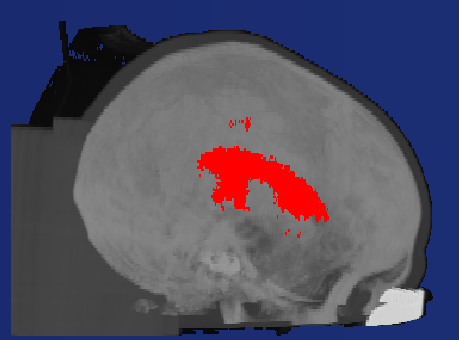
\includegraphics[width=\textwidth/2]{Logos/Seite.PNG}
\caption{Visualisierung des Ventrikels von der Seite} 
\label{fig:ventrikel_seite} 
\end{figure}
\begin{figure}[h] 
\centering 

\includegraphics[width=\textwidth/2]{Logos/Unten.PNG}
\caption{Visualisierung des Ventrikels von Unten} 
\label{fig:ventrikel_unten} 
\end{figure}
\begin{figure}[h] 
\centering 

\includegraphics[width=\textwidth/2]{Logos/Oben.PNG}
\caption{Visualisierung des Ventrikels von Oben} 
\label{fig:ventrikel_oben} 
\end{figure}



\todo{nutzerstudie variablen etc. erwähnen -> proseminar}
\todo{info über teilnehmer}
Im Rahmen der Evaluation der Benutzerfreundlichkeit des Verfahrens wurde eine kleine Nutzerstudie mit ... Teilnehmern durchgeführt. Bei dieser wurden den Probanden zunächst der Ablauf und die vom Benutzer erforderlichen Schritte um eine Visualisierung des Ventrikelsystems zu erhalten durch eine Vorführung durch den Interviewer gezeigt. Anschließend mussten die Teilnehmer selbst das eben gelernte anwenden und das Programm selber ausführen. Dabei bekamen sie, wenn sie nicht weiterwussten, Hilfe vom Versuchsleiter. Als Abschluss füllten die Probanden einen NASA-TLX Bogen zu der Aufgabe aus. Die durchschnittlichen Ergebnisse der einzelnen Kategorien wird in \autoref{tab: ergebnis_nasa} gezeigt.


\begin{table}[h]
\centering
\resizebox{\columnwidth}{!}{
 \begin{tabular}{| c | c | c | c |}
  \hline
  Kategorie & Gewichtung & Klicks & Wichtung \\ \hline
  Geistige Anforderung & 0&0 &0 \\ \hline
  Körperliche Anforderung & 0& 0& 0\\ \hline
  Zeitliche Anforderung &0 &0 &0 \\ \hline
  Leistung &0 &0 & 0\\ \hline
  Anstrengung &0 & 0& 0\\ \hline
  Frustration &0 &0 & 0\\ \hline 
 \end{tabular}
 }
\caption{Durchschnittlichen Ergebnisse des NASA-TLX Bogens}
\label{tab:ergebnis_nasa}
\end{table}


Der durchschnittliche Wert für die Gesamtbeanspruchung lag bei ... Personen ohne Programmiererfahrung ...

 
Trotz der Schwierigkeiten,  gaben die Probanden an, dass sie die Aufgabe mit einer guten ausführlichen Dokumentation auch alleine ohne Hilfe hinbekommen würden.


\todo{normale, schlanke etc. erwähnen plus sagen wie gut es funktioniert hat}





































































